%%%%%%%%%%%%%%%%%%%%%%%%%%%%%%%%%%%%%%%%%%%%%%%%%%%%%%%%%%%%%%%%%%%%%%%%
\begin{appendices}
\chapter{Appendix: conditional GAN}\label{chap:fcga)app}
%\appendix
\section{Performance}
\label{sec:app1}

%------------------------------------------------------------
\begin{figure}[b!]
\centering
\includegraphics[page = 2, width=0.49\textwidth]{figures/cGAN/pull_full}
\includegraphics[page = 3, width=0.49\textwidth]{figures/cGAN/pull_full} \\
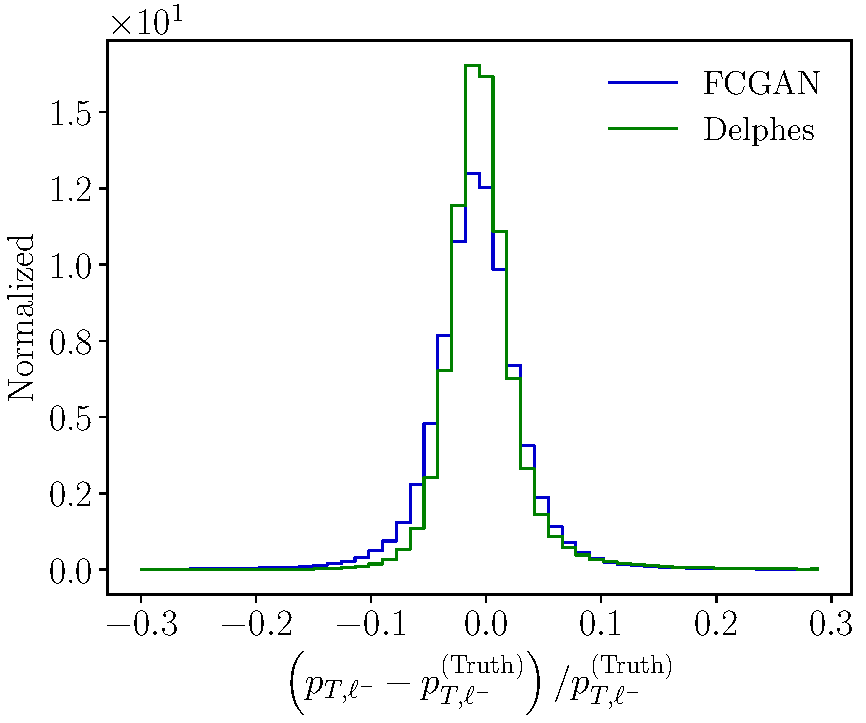
\includegraphics[page = 1, width=0.49\textwidth]{figures/cGAN/pull_full}
\includegraphics[page = 4, width=0.49\textwidth]{figures/cGAN/pull_full}
\caption{Normalized deviation between the FCGANned sample and truth (residual)
 for some of the kinematic variables.}
\label{fig:app_pull}
\end{figure}
%------------------------------------------------------------

While it is clear from the main text that the FCGAN inversion of the
fast detector simulation  works extremely well, we can still show some
additional standard measures to illustrate this. For instance, in
Fig.~\ref{fig:app_pull} we show the event-wise normalized deviation
between the parton-level truth kinematics and the \delphes and
FCGAN-inverted kinematics, for instance
%
\begin{align}
\frac{p_{T,j}^\text{(FCGAN)} - p_{T,j}^\text{(Truth)}}{p_{T,j}^\text{(Truth)}}
\qquad \text{and} \qquad
\frac{p_{T,j}^\text{(\delphes)} - p_{T,j}^\text{(Truth)}}{p_{T,j}^\text{(Truth)}} \; .
\end{align}
%
The events shown in these histograms correspond to the full phase
space inversion shown in Fig.~\ref{fig:distributions_FCGAN}, but from
the discussion in the main text it is clear that the picture does not
change when we invert only part of phase space.  As expected, we see
narrow peaks around zero, with a width in the $\pm 10\%$ range for the
jet momenta and much more narrow for the leptons, which are less
affected by detector smearing. For all distributions, but especially
the reconstructed $W$-mass, we see that the FCGAN reconstruction is
significantly closer to the parton-level truth than the \delphes
events are.

%------------------------------------------------------------
\begin{figure}[t]
\centering
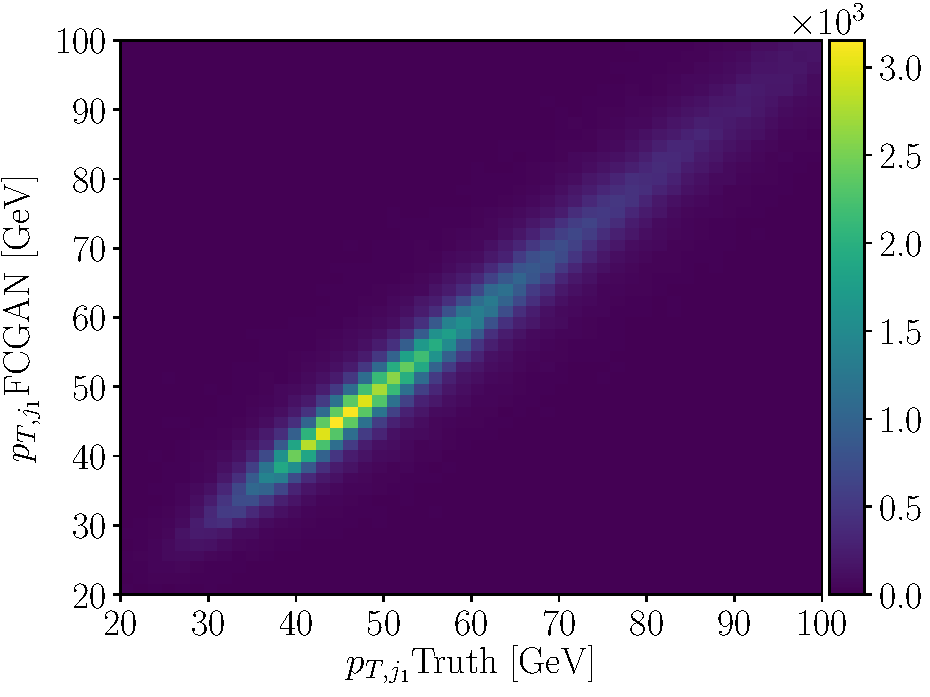
\includegraphics[page = 1, width=0.49\textwidth]{figures/cGAN/cGAN_pt1_corr}
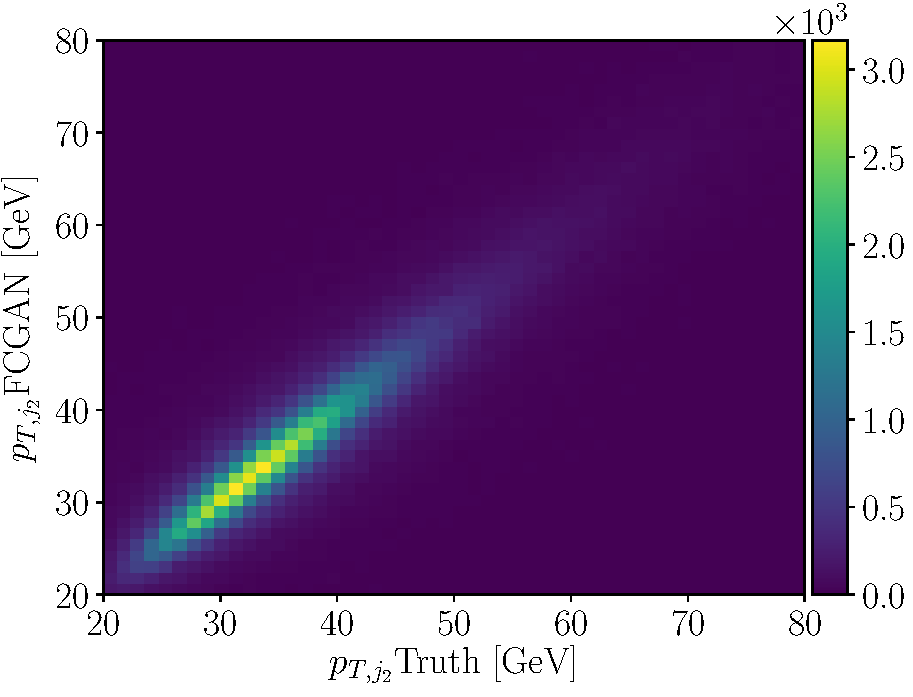
\includegraphics[page = 1, width=0.49\textwidth]{figures/cGAN/cGAN_pt2_corr}
\caption{Correlations between the FCGAN-inverted and parton-level truth
 kinematics, or migration matrix.}
\label{fig:app_2d}
\end{figure}
%------------------------------------------------------------

Finally, we show the migration matrix or correlation between true
parton-level and reconstructed parton-level events in terms of some of
the kinematic variables in Fig.~\ref{fig:app_2d}. Not surprisingly,
we observe narrow diagonal lines.

%%%%%%%%%%%%%%%%%%%%%%%%%%%%%%%%%%%%%%%%%%%%%%%%%%%%%%%%%%%%%%%%%%%%%%%%
\section{Staggered vs cooling MMD}
\label{sec:app}

The MMD loss is a two-sample test looking at the distance between
samples $x$, $x'$, drawn independently and identically distributed, in
terms of a kernel function $k\left(x, x'\right)$.  Implementations of
such a kernel, as given in Eq.~\ref{eq:kernels}, include a fixed
width or resolution $\sigma$.  We employ the MMD loss to reproduce the
invariant mass distribution of intermediate on-shell particles
$M_p$. A natural choice of $\sigma$ is the corresponding particle
width. However, this is inefficient at the beginning of the training,
when any generated invariant mass $M_G$ is essentially a random
uniform distribution. In that case $\left(x - x'\right)^2 \gg
\sigma^2$ for any $x, x' \sim M_G$, and Eq.~\ref{eq:MMD} reduces to
%
\begin{align}
\text{MMD}\left(k; M_G,M_P\right) \simeq \sqrt{\langle k\left(y,y'\right)\rangle_{y,y' \sim M_P}} \simeq \text{const} \; ,
\end{align}
%
and provides little to no gradient.

This can be avoided by computing the MMD loss using multiple kernels
with decreasing widths, so that the early training can be driven by
wide kernels.  A drawback of this approach is that only the small
subset of kernels with a resolution close to the evolving width of
$M_G$ gives a non-negligible gradient.

Alternatively, we can employ a cooling kernel, which we initialize to
some large value and then shrink to the correct particle width. This
is an efficient solution at all stages of the training.  A subtlety is
that the rate of the cooling has to follow the pace of the
generator in producing narrower invariant mass
distributions. Ultimately, we want to avoid hand-crafting the cooling
process, because it adds hyper-parameters we need to tune.  We use a
dynamic kernel width as a fixed fraction of the standard deviation of
the $M_G$ distribution.  This standard deviation as an estimate of the
width of $M_{G}$ can be replaced by any measure of the shape of
$M_{G}$, such as the full width at half maximum, and our tests show
that the performance is largely insensitive to the choice of the
fraction.

Yet another approach is based on the observation that the MMD kernel
test is not restricted to one-dimensional distributions
~\cite{GMMN,MomentMatching, MMDgen}.
This allows us to improve the invariant mass reconstruction by including
 additional physical information $x_i$ to the test, so that the
 discrepancy is not computed just between the samples $M_P$ and $M_G$
 of real and generated invariant masses, but rather between
 $(M_P, x_P)$ and $(M_G, x_G)$.
In the FCGAN spirit we therefore augment the batches of true and
generated invariant masses with one of
conditional invariant masses. From the same detector
information used to condition the generator and the discriminator, we
can extract the detector level invariant masses $M_D$ and accordingly
compute $\text{MMD}(k; (M_G, M_D), (M_P, M_D))$. Even tough
this does not represent a conditional MMD, training with multiple
kernels benefits from using the augmented batches. In
Fig.~\ref{fig:kernels_comparison} we compare the same invariant mass
distribution using these different MMD implementations.

%-------------------------------------------------
\begin{figure}[t]
\centering
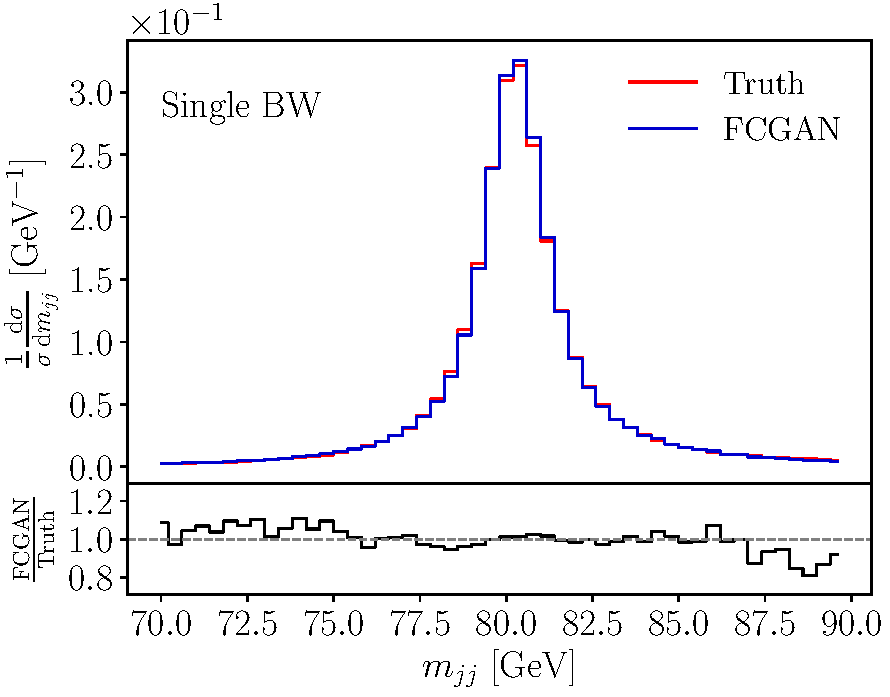
\includegraphics[page=1,width=0.49\textwidth]{figures/cGAN/single_1}
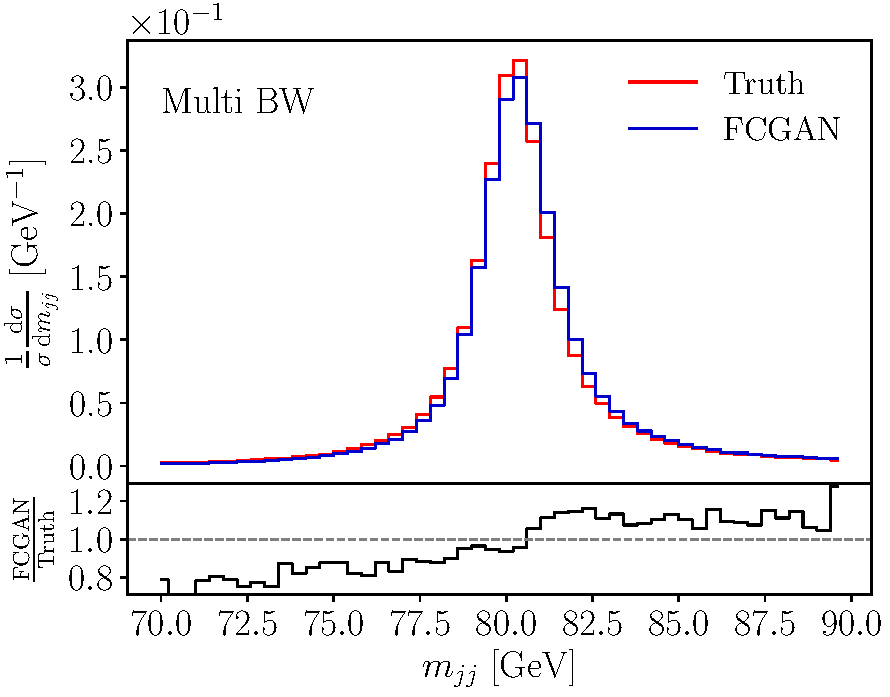
\includegraphics[page=1,width=0.49\textwidth]{figures/cGAN/multi_1}\\
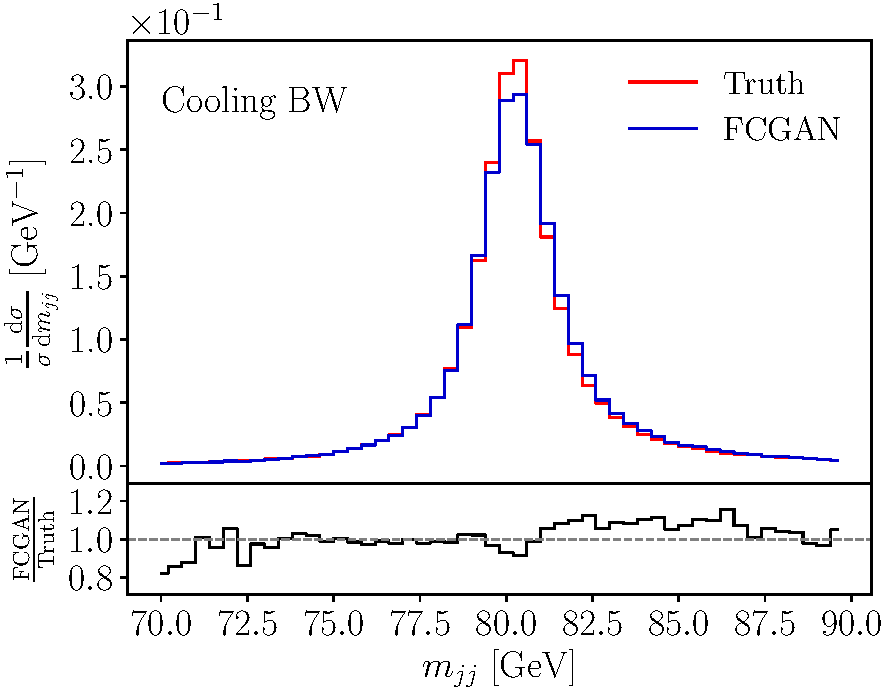
\includegraphics[page=1,width=0.49\textwidth]{figures/cGAN/cooling_1}
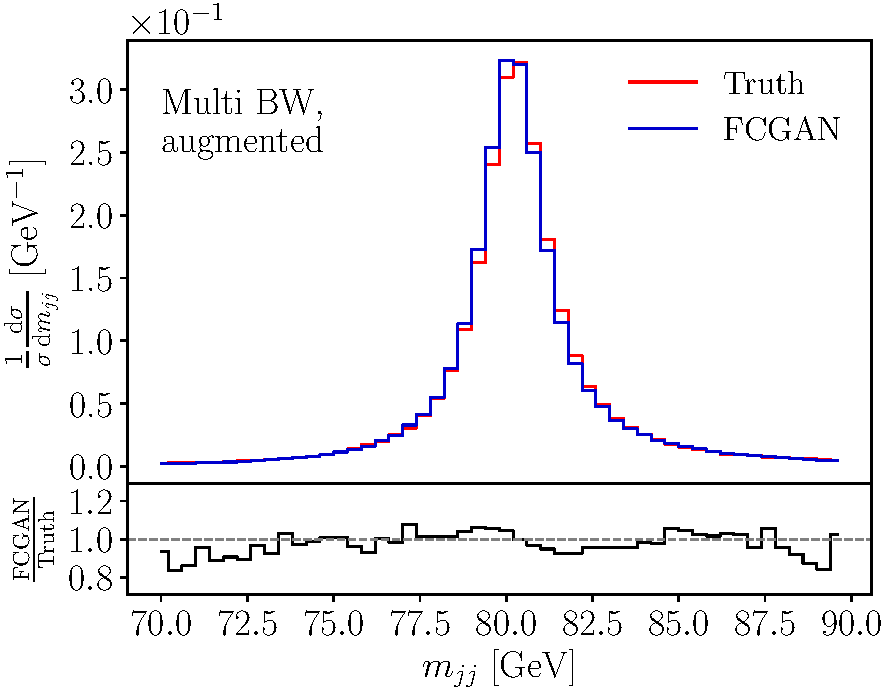
\includegraphics[page=1,width=0.49\textwidth]{figures/cGAN/combined_1}
\caption{Invariant jet-jet mass distribution for different MMD loss
  implementations: single kernel (upper left), multiple kernels (upper
  right), cooling kernel (lower left) and augmented multiple kernels
  (lower right).}
\label{fig:kernels_comparison}
\end{figure}
%-------------------------------------------------

\end{appendices}